\section{Chapter 3: Proposed Design}
The proposed design for this project will consist of the following:
\begin{itemize}
	\item A Front-end web application
	\item An API Gateway for the web app to access the Microservices
	\item Microservices are accessed through their own API
	\item The system created will consist of two different styles of database: a centralised DB and the ''traditional'' separated Db style associated with Microservice Architecture
\end{itemize}
The high level design of this system See figure \ref{fig:HighLvlAbstract}.
	\begin{figure}[h]	
		\caption{High Level Design}
		\label{fig:HighLvlAbstract}			
		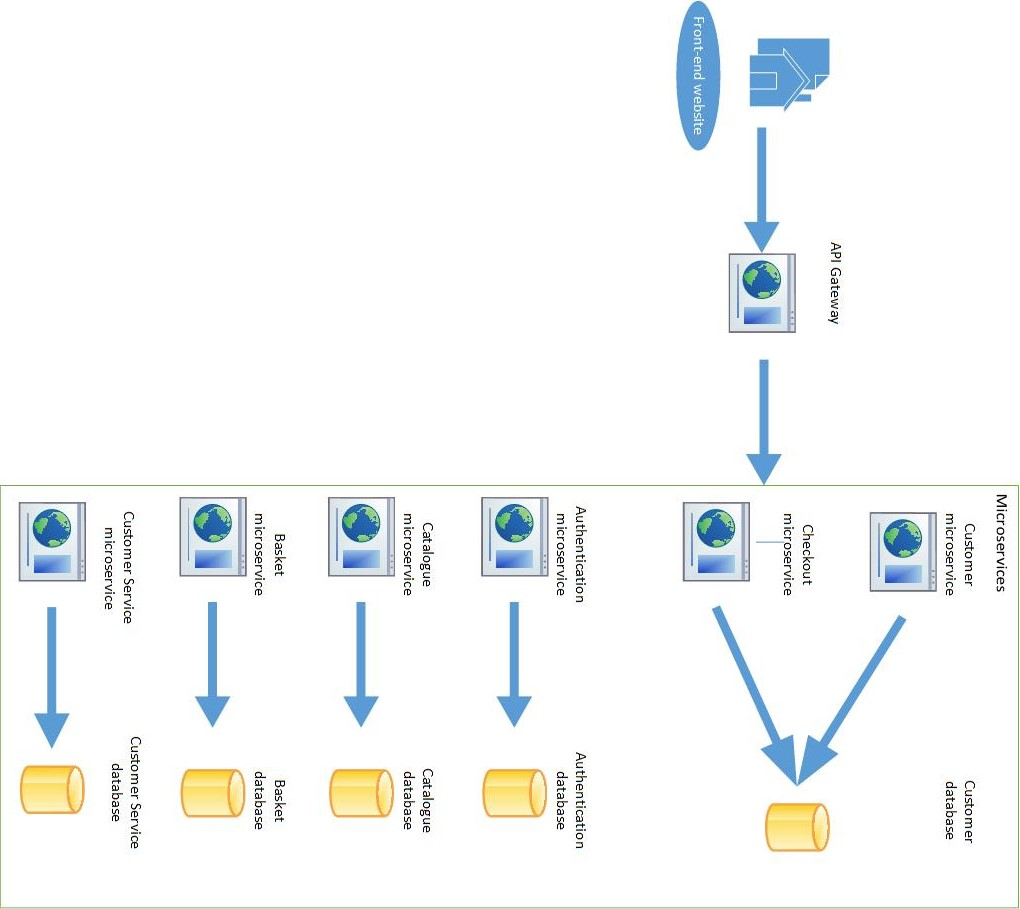
\includegraphics[height=12cm, width=15cm]{HighLevelAbstract}
	\end{figure}

This diagram shows how the front-end web system will interact with the Microservices. The website will be created using the MVC pattern. With each section of the UI needing to interact with a service(s) is done through the API Gateway to the microservices own API. 
An API Gateway will be chosen as the entry way for access to each Microservice. An API Gateway has been chosen as it seen as the best option to incorporate expansion - such as adding more Microservices, introducing different User-interfaces (Mobile version/Single Page Website etc.) this way the connectors, to each Microservice, are removed from the website. This prevent unnecessary complexity in the website instead having this present in the Gateway which will be more manageable.
 
From here Each Microservice will be accessed through its own API. That only the API Gateway will be able to access. Adding a level of protection and ensuring each Microservice is not coupled with the website. By incorporating API controllers, The RESTful implementation for each Microservice can be controlled. Removing any redundant ''verbs'' for each service. 
Although this Prototype will run mostly form a single machine. It is entirely possible for each Microservice to be running on a separate machine,, fully embracing the distributed system style. Also, the project will look into incorporating Docker to containerise each Microservice, API Gateway and the website. To explore this option and emphasise the requirement for a microservice architecture-system to be distributed.
\\
The bounded Context for this system will be: see figure \ref{fig:BoundedContext}
	\begin{figure}[h]
		\caption{Bounded Context}
		\label{fig:BoundedContext}
		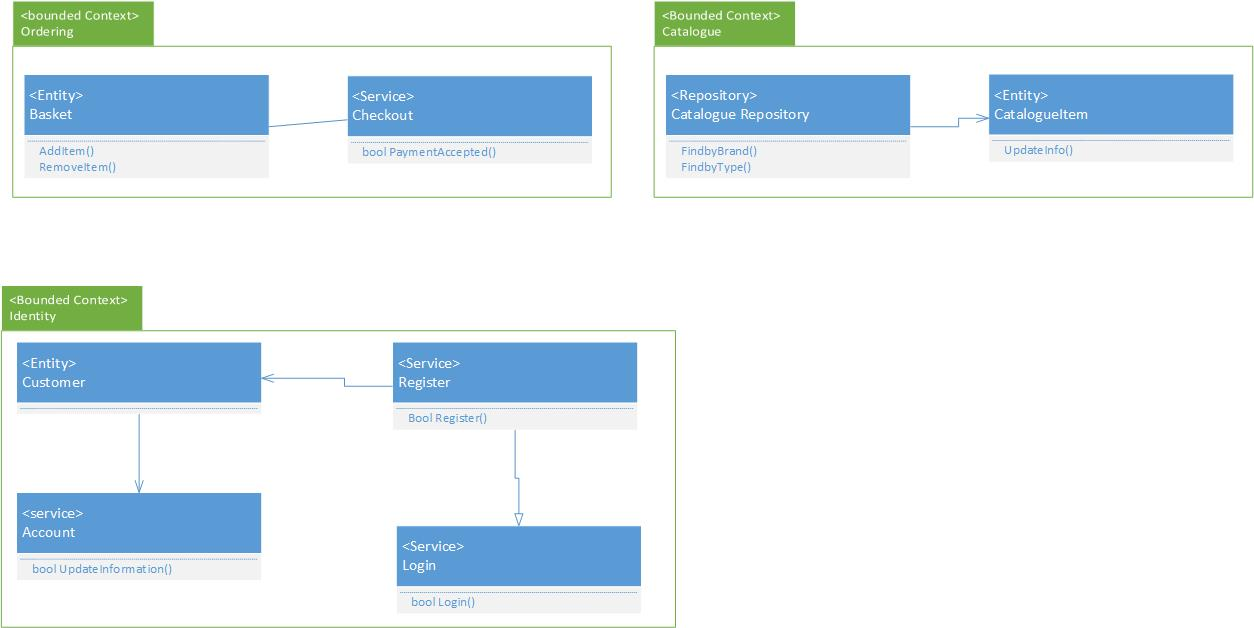
\includegraphics[height=10cm, width=16cm]{BoundedContexts}
	\end{figure}
There was three bounded contexts identified for this prototype:
\begin{itemize}
	\item Ordering\\
	This context covers the Basket Entity and Checkout Service. The Basket is the representation of a literal shopping basket/trolley that a customer will ''fill-up'' with selecting items. Naturally allowing the user to add, remove and update items they have added to their basket
	The Checkout is the representation of the user buying the items in the basket. As in the physical world, a customer will go to the checkout to buy the items they want. Here is where the transaction will occur in the system.
	\item Catalogue\\
	The Catalogue context will contain all the information for each item available for purchasing. Representing a warehouse, the repository was identified to be used here that store all catalogue items. Each individual Item is also recognised and represented as an individual entity. Each item has its own Entity. And the Repository consists of these Entities.
	\item Identity\\
	This is the representation of the customer and all associations with the customer. Where the customer will be an entity stored within the database that will contain the personal information of each person who has registered with the website. This will also be what the service Account mostly comprises of: the ability for customers to edit their information as when required. The login and register services are self explanatory: the register service is the portal for users to register as ''customers'' with inputting the necessary information, this is where the user's customer entity is created and stored in the customer database. Login service is the portal for users to login using the password they created and Email address they registered with.
\end{itemize}

NOTE: For the purposes of this prototype the registers users information will be generic.
\pagebreak
\\The chosen interfaces for each Microservice: see figure \ref{fig:MSAInterfaces}\\
\begin{figure}[h]
	\caption{Interface}
	\label{fig:MSAInterfaces}
	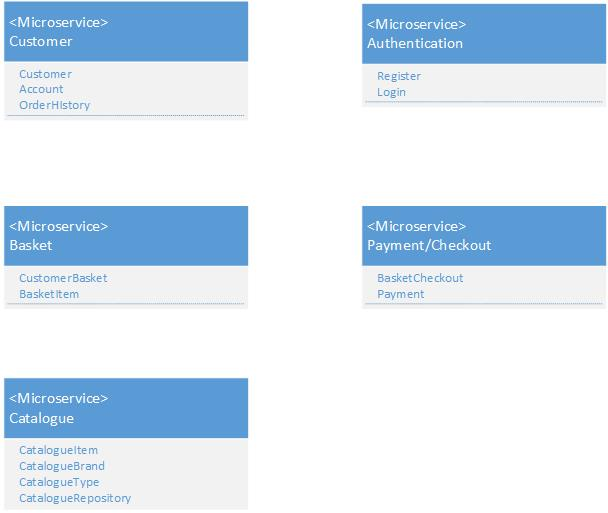
\includegraphics[height=15cm, width=15cm]{MicroserviceInterfaces}
\end{figure}
This diagram shows the composition of each microservice
\begin{itemize}
	\item Customer Microservice\\
	This contains all the classes needed to represent this microservice. Customer class that stores all the users personal information, the customer ID being the primary key of the record automatically generated when the user registers. The order history class is the representation of each order placed by the user. Note to be taken that each order may comprise multiple items.   Account class is the collection of all previous orders placed and the user's information. Allowing the user to view their previous orders and edit their information.
	\item Authentication Microservice\\
	This contains the classes for a user to login and register. The basis for the authentication for this system. The register Class forms the entity that will compose the customer object from the respective class.
	\item Basket Microservice\\
	This interface's classes are linked with each other. Each item added to the basket will be created as an object of the BasketItem class and the customer basket will contain all the BasketItems every time one is added/removed/edited.
	\item Checkout Microservice\\
	\item Catalogue Microservice\\
	This microservice will house the entire catalogue of items available for sale. Each Catalogue Item will be created as an individual object, each being added to the catalogue repository that will be used by the website, by consuming the Catalogue API, to display each catalogue item to the user. The CatalogueBrand and CatalogueType classes will be used to search for specific items based on brand or type.
\end{itemize}
\pagebreak
The microservices will interact in the following manner: see figure \ref{fig:MSAInteractions}\\
\begin{figure}[h]
	\caption{Interactions}
	\label{fig:MSAInteractions}
	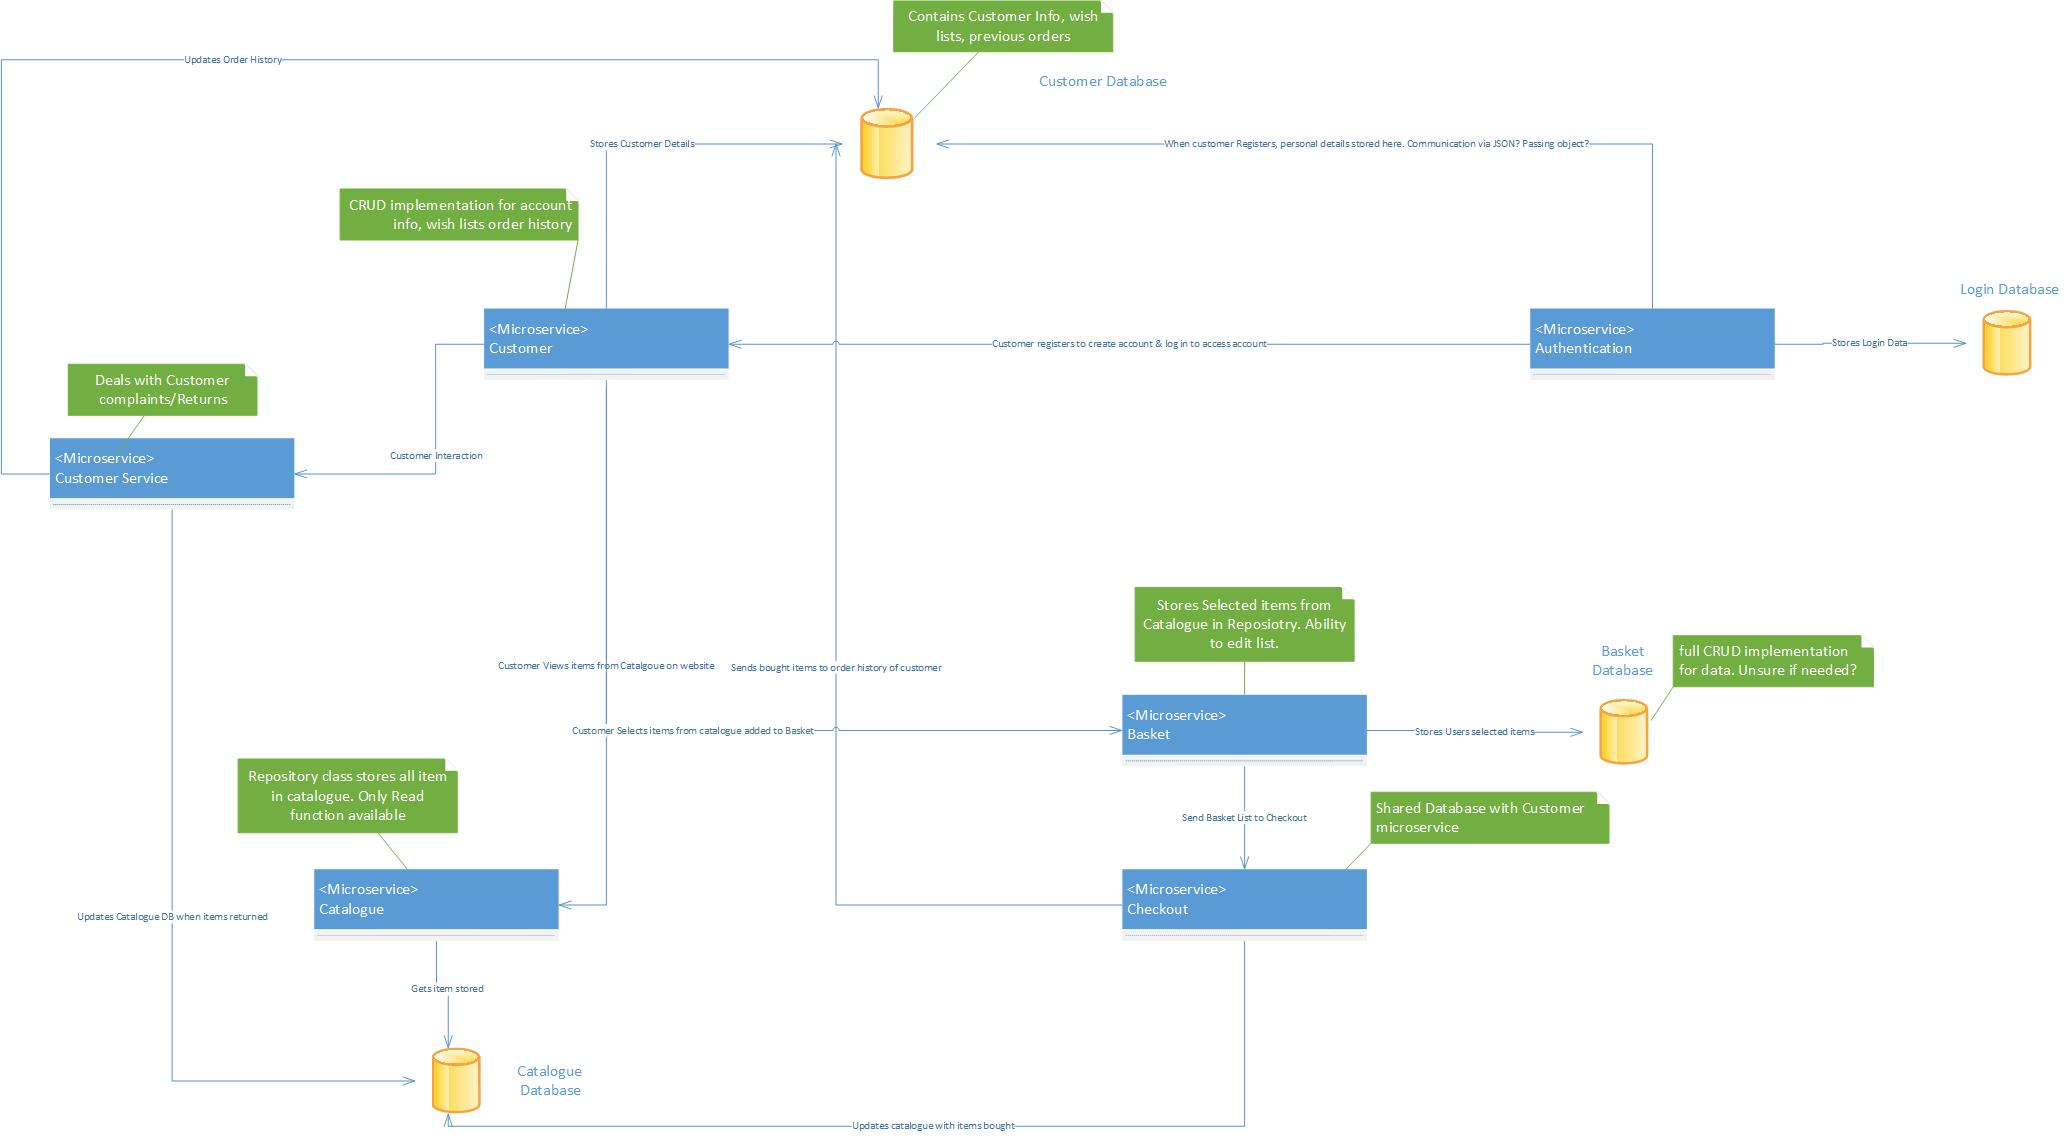
\includegraphics[height=15cm, width=17cm]{ServiceInteraction}
\end{figure}
Microservice Interaction is complicated. As can be seen by the diagram. To date, a more suitable modelling diagram for microservice interaction has not been found. Microservice Interaction is thus:
\begin{itemize}
	\item Authentication Microservice\\	
	This microservice will store the login details within its own databases, Email and password, and sending the full set of information entered to the customer Database.
	When a user enters their login credentials, this is checked with current records in the login DB and either successful or not.
	\item Customer Microservice\\
	Gets the customer information from authenticate service and stores it within its own database.
	Receives the object of bought items from the checkout service and stores them as part of the order history.
	When a user creates a ticket for the customer service Microservice this service sends the customer ID to be attached to the ticket for identification purposes.
	\item Basket Microservice\\
	Receives an updated object for an order if anything was changed with a previous order such as an item returned etc. The record in the customer DB is updated to reflect changes.
	\item Checkout Microservice\\
	Receives the repository of basket items from the Basket microservice
	Sends the basket repository, from a successful checkout process, to the customer microservice.
	\item Catalogue Microservice\\
	Gets all catalogue items from the database to be viewed. 
	Receives updates on items from customer service and Checkout Microservices when stock numbers increases/decreases and the amount.
	\item Customer Service Microservice
	Receives customer ID from Customer Microservice to for customer ticket.
	Sends updated order to customer if anything has been changed.
	Sends updated stock count of items from an order to the Catalogue Microservice if anything has changed.
\end{itemize}
\pagebreak
Class diagrams for the Microservices: figure \ref{fig:AuthentClass}, figure \ref{fig:BaskClass}, figure \ref{fig:CatalogueClass}, figure \ref{fig:CheckoutClass}, figure \ref{fig:CustomerClass}.